
%(BEGIN_QUESTION)
% Copyright 2015, Tony R. Kuphaldt, released under the Creative Commons Attribution License (v 1.0)
% This means you may do almost anything with this work of mine, so long as you give me proper credit

In this process, ammonia vapor and nitric acid are combined in a chemical reactor vessel to form ammonium nitrate, one of the principal ingredients of synthetic fertilizer.  A flow controller (FIC-36) regulates the flow of ammonia vapor into the reactor:

$$\includegraphics[width=15.5cm]{i0008rx01.eps}$$

Suppose the last instrument technician to calibrate flow control valve FV-36 made a mistake, such that the valve stem position is 5\% further open than it should be at all signal values.  For example, if the controller sends a 25\% (8 mA) signal to the control valve, it actually opens up to 30\%.

\vskip 10pt

Describe in detail the effect this mis-calibration will have on the regulation of ammonia vapor flow.

\vskip 20pt \vbox{\hrule \hbox{\strut \vrule{} {\bf Suggestions for Socratic discussion} \vrule} \hrule}

\begin{itemize}
\item{} Perform a ``thought experiment'' where someone attaches a wooden block to the accelerator pedal of your car without your knowledge, so that the accelerator pedal will be pressed down further than you think it is for any given foot position.  How will this affect your actual driving speed as you attempt to obey the speed limit?
\item{} Why would a {\it regulated} flow rate of ammonia vapor be important in a process such as this?
\item{} Explain why three pH transmitters (AIT-28a, AIT-28b, AIT-28c) are used to measure the neutralizer's effluent pH instead of just using one transmitter.
\item{} Suppose the positioner on FV-25 fails so that the valve opens wide.  How will this fault affect the liquid level in V-7 (the rundown tank)?
\item{} Suppose the circuit breaker feeding electrical power to the VFD on pump P-105 trips.  How will this fault affect variables in this process?  Will any loop controllers attempt to compensate for the fault by responding with changes in output signal?
\item{} LT-35 is a ``bubbler'' style of level sensor, slowly bubbling compressed air out the end of a submerged tube.  The more liquid inside scrubber V-5, the more compressed air ``backpressure'' builds up inside the bubble tube, causing the pressure-sensing transmitter to register a greater liquid level.  Suppose this ``bubble tube'' plugs at its very end (submerged inside the tank).  How will this fault affect the actual level inside the scrubber?
\end{itemize}

\underbar{file i04388}
%(END_QUESTION)





%(BEGIN_ANSWER)

%(END_ANSWER)





%(BEGIN_NOTES)

\filbreak \vskip 20pt \vbox{\hrule \hbox{\strut \vrule{} {\bf Virtual Troubleshooting} \vrule} \hrule}

\noindent
{\bf Predicting the effect of a given fault:} present each of the following faults to the students, one at a time, having them comment on all the effects each fault would produce.

\begin{itemize}
\item{} 
\item{} 
\item{} 
\end{itemize}


\vskip 10pt


\noindent
{\bf Identifying possible/impossible faults:} present symptoms to the students and then have them determine whether or not a series of suggested faults could account for all the symptoms, explaining {\it why} or {\it why not} for each proposed fault:

\begin{itemize}
\item{} Symptom: {\it }
\item{}  -- {\bf Yes/No}
\item{}  -- {\bf Yes/No}
\item{}  -- {\bf Yes/No}
\end{itemize}


\vskip 10pt


\noindent
{\bf Determining the utility of given diagnostic tests:} present symptoms to the students and then propose the following diagnostic tests one by one.  Students rate the value of each test, determining whether or not it would give useful information (i.e. tell us something we don't already know).  Students determine what different results for each test would indicate about the fault, if anything:

\begin{itemize}
\item{} Symptom: {\it }
\item{}  -- {\bf Yes/No}
\item{}  -- {\bf Yes/No}
\end{itemize}


\vskip 10pt


\noindent
{\bf Diagnosing a fault based on given symptoms:} imagine the nozzle inside of LV-35's positioner plugs up in this system, causing that control valve to open fully (don't reveal the fault to students!).  Present the operator's observation(s) to the students, have them consider possible faults and diagnostic strategies, and then tell them the results of tests they propose based on the following symptoms, until they have properly identified the nature and location of the fault:

\begin{itemize}
\item{} Operator observation: {\it LG-31 reads a high level -- 88\% full}
\item{} Signal from LT-35 agrees with LG-31 -- 18.1 mA
\item{} LIR-30 agrees with LG-31 -- 87\%
\item{} LIC-35 is in automatic mode, with the output displaying 0\%
\item{} LIC-35 output signal is 3.9 mA
\end{itemize}
%INDEX% Basics, control loop troubleshooting: determining effect of specified fault(s)
%INDEX% Process: ammonium nitrate production (realistic P&ID shown)

%(END_NOTES)


